% ---------------------------------------------------------------------------
%  Section 2: Impact
% ---------------------------------------------------------------------------

\TOWRITE{ALL}{Proofread 2 Impact1.4 Ambition pass 2}

\section{Impact}
\label{sec:impact}

%\TOWRITE{Simula}{Hans Petter and Valeriya will make a second iteration on the impact section for Friday}

\TOWRITE{ALL}{Check and complement the impact section}

The project, with its ambitious vision, general and broad approach, and 
challenging work plan, will offer the opportunity to all partners and beyond 
to complement their research expertise with methodologies and tools not 
available at their institutions. It will provide pivotal aspects needed 
for the development of a new generation of high-efficient scientific leaders 
with an open and constructive attitude toward collaborative interdisciplinary 
research and innovation. The diverse nature of the objectives composing the 
project will also be taken into account to design a successful and multiform 
dissemination and exploitation strategy.

\subsection{Expected Impacts}

\eucommentary{Please be specific, and provide only information that applies
to the proposal and its objectives. Wherever possible, use quantified
indicators and targets.\\
Describe how your project will contribute to:\\
-- the expected impacts set out in the work programme, under the relevant topic
(including key performance indicators/metrics for monitoring results and impacts);\\
-- improving innovation capacity and the integration of new knowledge
(strengthening the competitiveness and growth of companies by developing
innovations meeting the needs of European and global markets; and, where
relevant, by delivering such innovations to the markets;\\
-- any other environmental and socially important impacts (if not already
covered above).\\
Describe any barriers/obstacles, and any framework conditions (such as
regulation and standards), that may determine whether and to what extent
the expected impacts will be achieved. (This should not include any risk
factors concerning implementation, as covered in section 3.2.)}

\subsubsection{Impacts as Listed in the Work Programme}

The following table shows how \TheProject  addresses the specific impacts
listed in the work programme
\footnote{We will survey mathematical departments
(and relevant members of other departments 
during year 1 and again during year 4 to gauge the awareness of the 
existence and capabilities of \TheProject and its components, and to collect
statistical data for estimating Key Performance Indicators listed
in the table. The success factor is a positive change between the two surveys. 
Other measures not listed in the table include activity on the relevant mailing 
lists and forums and the numbers of downloads (though this is hard to measure 
for many reasons)}.

%\tablehead{}
\begin{supertabular}{|m{.42\textwidth}m{.52\textwidth}|}\hline\hline
\multicolumn{2}{|m{.94\textwidth}|}{\textbf{1. More effective collaborations between researchers}}\\\hline

  \TheProject will strengthen collaborations between European scientific community in
  different branches of mathematics, through a development of the common e-infrastructure
  by bringing together previously separated software and databases, and building links with
  scientific communities in other disciplines (biology, physics, astronomy) that will use
  this e-infrastructure. The scientific community will considerably increase, by
  integrating new actors both from academic and non-academic sector. 
& Key performance indicators:
  \begin{compactenum}
  \item Number of researches in the mathematical scientific community 
        using VREs based on \TheProject.
  \item Number of researches in other disciplines (natural sciences, 
        engineering, etc) and industry using VREs based on \TheProject.
  \item The number of attendees of our training and dissemination events.
  \item Number of collaborative (i.e. across institutions) publications 
        using VREs based on \TheProject.
  \end{compactenum} \\\hline

  \hline\multicolumn{2}{|m{.94\textwidth}|}{\textbf{2. Higher efficiency and creativity in research, higher productivity of researchers  thanks to reliable and easy access to discovery, access and re-use of data}}\\\hline

  The development of a new integrated tool, replacing %3 why 3? Commented out. AK
    previously separated tools, a possibility of real time data sharing, data re-use and
    simultaneous working will allow substantial gains in time and in efficiency, and, by
    consequence, higher productivity of researchers. Moreover, the exchange of best
    practice (such as regular code audit) will have an important impact on research
    quality. Finally, the unique tool will allow considerable reduction of further 
    research costs.

 &

  Key performance indicators :
  \begin{compactenum}
\item The e-infrastructure developed by the end of the project will allow to reduce
the time of research by up to X\% and to increase the productivity of researchers by 
up to X\%
\item Due to the dissemination of best practices, research quality will considerably 
increase, and the number of errors will be reduced.
\item Better traceability and discoverability of research outputs.
\item Considerable reduction of research costs.
\end{compactenum}

\\\hline
\hline\multicolumn{2}{|m{.94\textwidth}|}{\textbf{3. Accelerated innovation in research via an integrated access to digital research resources, tools and services across disciplines and user communities}}\\\hline

An integrated access to digital research
resources and tools that \TheProject will provide will clearly help to
accelerate innovation in research across disciplines and communities.

The integrated tool will meet the needs of all disciplines covered by
the project and will help to overcome commonly found obstacles in
both academic and non-academic research in these disciplines. Industrial
actors, actively involved in the project, will directly benefit from
the project results. &

Key performance indicators :

\begin{compactenum}
\item Emergence of new, improved research methods and workflows 
in several disciplines using the tool. % for example, virtualised experiments
\item Resolving of series of problems inherent to industrial actors in several disciplines.
\item The speed of resolution of issues across components (e.g. bugs 
reported by \Sage users and problems encountered by \Sage developers 
integrating \GAP being resolved by the \GAP team. 
\item The number of components/libraries that are compatible with the \TheProject user interface.
\item The number of components/tools/packages that may be used in parallel
programs, or which incorporate parallelism in their own routines.
\item The number of joint publications and grant applications arising from the project
\item The number of external collaborators and contributors to \TheProject.
\end{compactenum}
\\\hline
\hline\multicolumn{2}{|m{.94\textwidth}|}{\textbf{4. Researchers able to process structured and qualitative data in virtual and/or ubiquitous workspaces}}\\\hline
\TheProject will enable researchers to process
different kind of  data due to an integrated tool interconnected
with databases. Efficient data storage will allow further exploitation
and  re-use of mathematical data for further calculations and thus make
data processing more efficient.
 &
Key performance indicators:
\begin{compactenum}
\item Number of data sets made available in mathematical databases supported by \TheProject.
\item Number of \TheProject components that are able to access those data sets, where relevant.
\item Number of remote queries to retrieve information from data sets hosted by project members.
\end{compactenum}
\\\hline

\hline\multicolumn{2}{|m{.94\textwidth}|}{\textbf{5. Increased take-up of collaborative research and data sharing by new disciplines, research communities and institutions}}\\\hline

The project will clearly enhance a take-up
of collaborative research and data sharing by and between new
disciplines and research communities. Those communities already using 
parts of the tool, will be enlarged, involving more and more industrial
actors and young scientists.

By developing the tool, it will reinforce collaborations between
different branches of mathematics (both pure and applied). Once
developed, the tool will be opened for research in various disciplines,
such as biology, physics, astronomy etc. &
Key performance indicators :

\begin{compactenum}
\item Increase in collaboration and data sharing between different communities in
  mathematics.
\item Increase in collaboration and data sharing between research communities in other
  disciplines.
\item Increase in the number of users and research communities using the tool.
\item Increase in the number of publications citing \TheProject and its components,
      and in the number of institutions and disciplines exhibited in these publications
      (although the timescales of publishing in some disciplines, including mathematics,
      mean that this will be very much a lagging indicator).
\end{compactenum}
\\\hline
\end{supertabular}


\subsubsection{Improving innovation capacity and the integration of new knowledge}


Innovations developed by the \TheProject project will meet the needs of the
following ecosystem participants:

\begin{compactenum}
\item Device/module vendors: hardware manufacturers, equipment
manufacturers of smartphones, tablets, laptops;
\item Network providers: service providers, network infrastructure
vendors (such as Avaya, Juniper, Extreme, Cisco, et al.);
\item Platform providers;
\item Cloud service providers: Software-as-a-Service,
Platform-as-Service, Infrastructure-as-a-Service;
\item Systeme integrators: end-to-end integration services and
value-added services (such as Accenture, HP, IBM, et al.)
\item End users: research communities; stakeholders in IT, healthcare, 
education, aeronautics, and other areas.
\end{compactenum}
Industrial stakeholders will be directly involved in the project and
the VRE development, so that the tool will be exactly tailored to their
specific needs as well as to the needs of the scientific community.
Moreover, this will allow short time-to-market and will facilitate
the technology uptake.

In the next table we have specified different market needs, and the
ways we will address each of them:

%\begin{flushleft}
\tablehead{}
\begin{supertabular}{|m{.30\textwidth}|m{.67\textwidth}|}
\hline
\centering Market needs &
\centering\arraybslash How the project will address these needs\\\hline
Performance gain &
The toolkit will enable its users to combine functionality from several major
open-source mathematical software systems and problem-oriented programming 
languages (including mainstream tools such as Python) in a modern integrated environment) on the majority of currently popular hardware platforms 
and operating systems.
\\\hline
Infrastructure capacity: newly built infrastructures with fast broadband
connections are well positioned for adopting our products &
\TheProject will allow different groups of users to collaborate and work simultaneously on the same document, and
thus providing a considerable gain in efficiency.\\\hline
Low scaling costs &
An open source architecture brings affordability: people and
organisations donate efforts towards common goals, and small organisations can
gain access to equipment and research talents otherwise only affordable by
the largest companies. Resources integration will reduce considerably the
time and the costs of operations.\\\hline
Going beyond limitations of interconnect technology &
An open source architecture enhances creativity due to the potential to
attract best minds from a wide pool of people to solve a problem\\\hline
Enabling new applications and features &
Through a series of connections that will be created between previously
separated tools, and data interoperability, \TheProject will enable new
applications and features. All derived VREs are new applications, with new features.\\\hline
Early time-to-market (TTM): companies are looking for solutions that
would improve the speed at which they can procure services to bypass
traditional information technology departments &
The speed of development will improve tremendously due to the new
collaborative features. Liaising with industrial stakeholders during
the development will allow to deliver a tool the suits their needs in
the best possible way, thus speeding-up the time-to-market and technology 
uptake.\\\hline
Easy-to-use service: first-time experiences are crucial to gain
acceptance &
We will design an ergonomic multi-user web-based graphical user
interface, following web standards to best support a large array of
browsers, including cell phones and tablets. We will explore
opportunities for integration in interactive boards, as an aid for
teaching and collaborative research.
\\\hline
\end{supertabular}
%\end{flushleft}

\subsubsection{Other Impacts (Environmental and Socially Important Impacts)}


We start from \Sage's mission statement: ``Creating a viable free open
source alternative to \Magma, \Maple, \Mathematica and \Matlab'' but
need to go beyond that goal, and make \TheProject a new reference
tool, that is deployed across science. To be successful our VREs will
need to provide much more than can be done through closed source
commercial systems. Large scale collaborative development is the key
to this goal, both on software and research, but coordination and
projection of vision is still crucial for success. We will focus on
the young generation, which will constitute its future users, for
example by producing learning materials for the so called ``Generation
Y''. ``Generation Y'' is expected to account for 30\% of the total
projected population in 2025, and will be the key influencer for
change in workplace habits, caused by such features as easy
adaptability to new technologies and social media, commonly attributed
to this generation.  \TOWRITE{??}{May we add some reference to support
  this statement?}

\TOWRITE{AK}{This section needs to be extended} 

\subsubsection{Potential Barriers to Impact}

The following barriers to impact will be addressed and overcome using the mitigation
strategies provided. These are distinct from the risks to project delivery
detailed in Section~\ref{sec:risks}.
\TOWRITE{ALL}{Some other barriers? Maybe lack of contribution from community to OpenDreamKit?}
\paragraph{Table 2.1: Barriers to Impact}

\ \\

\begin{longtable}{ | p{10cm} | c | }\hline
{\bf Barrier description } & {\bf Risk level } \\ \hline \hline
%{\bf  }                         & {\bf No }                &{\bf  level } {\bf       }    \\
& \\ 
{\bf Users will not use the new VRE environment}       &  High       \\ 
    &  \\
    \hline
\multicolumn{2}{| p{14.5cm}|}{
{\bf Contingency Plan:}  
A major concern in any proposal of this kind is that the resulting
tools will not be adopted by users. This is a particular concern with
such 'tradition-based' community as mathematicians.  This project has two pathways to tackle this:
(1) \TheProject is based on prior work, which \emph{already} has users;
(2) \TheProject will be integrated into the \Jupyter and \Sage, which \emph{already} have a significant user base;
(3) An end-user group formed at the beginning of the project by the representatives from different disciplines and sectors will provide valuable advice on real user needs throughout the project and assist in providing \TheProject sustainability.

In addition, the project's communication, dissemination, and
exploitation strategy will evolve throughout the project's implementation to
ensure that stakeholder communities are fully aware of the project's
progress, potential benefits, and innovative capacity and are engaged
in the integration of the final results.
}\\
\hline
&  \\
{\bf Dominance of competing frameworks  }  &  Medium        \\
 &  \\
\hline 
 \multicolumn{2}{| p{14.5cm}|}{
{\bf Contingency plan:}  
  Our strategy is to engage with  users  and attract new users at the very beginning
of the project, understand their requirements and design the domain-specific tools.
An international advisory
board will allow us to coordinate with the related research activities within and outside of Europe
and to promote our framework internationally. 
}
\\
\hline
\end{longtable}
\TOWRITE{All and NT}{Is dominance of competing frameworks really an issue? Is there anything out there AS GOOD as OpenDreamKit? Would be good to have more than just one barrier though.}



\subsection{Measures to Maximise Impact}
\TOWRITE{ALL}{go through the section and add specific input, relevant to your organisation on dissemination / exploitation activities}
The overall objectives of the dissemination and exploitation strategy are based on the project's core values, which are to improve the productivity of researchers in mathematics and connected fields by providing them with a unique virtual toolkit for a collaborative research tailored to their needs and requirements both during the project period and after the project completion.

\subsubsection{Dissemination and Exploitation of Results}
\label{subsubsect:dissemination}
\eucommentary{-- Provide a draft 'plan for the dissemination and exploitation
of the project's results'. The plan, which should be proportionate to the
scale of the project, should contain measures to be implemented both during
and after the project.\\
Dissemination and exploitation measures should address the full range
of potential users and uses including research, commercial, investment,
social, environmental, policy making, setting standards, skills and
educational training.\\
The approach to innovation should be as comprehensive as possible,
and must be tailored to the specific technical, market and organisational
issues to be addressed\\
-- Explain how the proposed measures will help to achieve the expected impact of the
project . Provide a draft business plan for financial sustainability as stated in the Part
E of the Specific features for Research Infrastructures of the Horizon 2020 European
Research Infrastructures (including e-Infrastructures) Work Programme 2014-2015.\\
-- Where relevant, include information on how the participants will
manage the research data generated and/or collected during the
project, in particular addressing the following issues:
What types of data will the project generate/collect? What
standards will be used? How will this data be exploited and/or
shared/made accessible for verification and re-use (If data cannot
be made available, explain why)? How will this data be curated and preserved?\\
-- Include information about any open source software used or developed by the
project.\\
You will need an appropriate consortium agreement to manage (amongst other things)
the ownership and access to key knowledge (IPR, data etc.). Where relevant,
these will allow you, collectively and individually, to pursue market opportunities
arising from the project's results.\\
The appropriate structure of the consortium to support exploitation is addressed
in section 3.3. \\
-- Outline the strategy for knowledge management and protection. Include measures to
provide open access (free on-line access, such as the ``green'' or ``gold'' model) to
peer-reviewed scientific publications which might result from the project.\\
Open access publishing (also called 'gold' open access) means that an article is
immediately provided in open access mode by the scientific publisher. The associated costs
are usually shifted away from readers, and instead (for example) to the university or
research institute to which the researcher is affiliated, or to the funding agency supporting
the research.\\
Self-archiving (also called ``green'' open access) means that the published article or the
final peer-reviewed manuscript is archived by the researcher - or a representative - in an
online repository before, after or alongside its publication. Access to this article is often -
but not necessarily - delayed (``embargo period''), as some scientific publishers may wish to
recoup their investment by selling subscriptions and charging pay-per-download/view fees
during an exclusivity period.}


The dissemination and exploitation strategy will be
presented in the dissemination and exploitation plan, prepared by the
Coordinator within \TOWRITE{All}{Add reference to task that produces
  dissemination and exploitation plan} the specifically designed WP
and implemented with the help of all partners. The planned activities
will bear in mind the project's scientific and societal impacts, and
build throughout the project to ensure that stakeholder communities
(1) are fully aware of the project and its potential benefits, (2)
engaged in integration of the VRE in their professional activities,
and (3) contribute to the sustainability and improvement of the
VRE. 

We summarise the dissemination activities
and how they will help to achieve the expected impact among our
stakeholders and target audiences in Table~\ref{table:dissem-plan}.

%% HF got to here reviewing 

%Three types of impact are possible with our dissemination and
%communication activities: (1) people or organizations are informed
%about \TheProject; (2) people or organizations act and use our conclusions
%or results; (3) people or organizations contribute and help to develop
%or improve the research infrastructure. The second form of impact
%supposes that parties understand the messages. The third form supposes
%learning, which is a very high level of impact. In the following table,
%we have listed how the proposed measures will help to achieve the
%expected impact among our stakeholders and target audiences.

\begin{table}
\begin{supertabular}{|m{3cm}|m{1cm}| m{7cm} | m{2cm}|}
\hline
Dissemination goal &
Target audience&
Dissemination method &
Timeframe and frequency  \\\hline
Project identity and profile &
T1-T6
&
Website; flyers/leaflets; videos.
& 
Throughout project, continuous \\\hline
Broad dissemination &
T3, T4, T6, T7 
&
Biannual e-newsletters; press releases; information database; social networks and platforms; news  in Nature and other editions in other disciplines; lectures in high schools led by PhD students.
& 
Throughout project, quarterly \\\hline
Knowledge transfer, information exchange&
T1,T2, T3
&

Organisation of 10 technical workshops; 10 scientific trainings/year; training of at least 100 PhD students for the infrastructure usage; publications in social aspects; software demonstration during conferences; workshop for PhD students in Africa; participation at the workshop 'Sage and women' in US; participation in international conferences like FPSAC, ISSAC, or the international congress of mathematical software; regular participation in annual Python conference; organising at least 8 scientific trainings for other scientific communities/projects; news  in Nature and other editions in other disciplines; certification by technology clusters.
& 
Throughout project, continuous  \\\hline
Demonstration of advantages and possible applications &
T1-T4
&
Organisation of 10 technical workshops; participation in annual Python conference.
& 
Biannually \\\hline
Uptake of the VRE by new users &
T2-T4
&
White papers; organise at least 8 scientific trainings for other scientific communities/projects; presentation at international conferences; 5 MooCs designed to master students; integration of project results into Master courses and into teacher training courses.
& 
Mo24-, at relevant milestones \\\hline
Sustainable development beyond the project &
T1-T4
&
Policy events; white papers; participation at conferences.
& 
Mo24-, at relevant milestones \\\hline
\end{supertabular}

\smallskip
{\bf Key for the ``Target Audience'' column:}
\begin{compactenum}
\item[T1] Scientific community in mathematics and related fields 
     (experienced researchers, under-/graduate/post-graduate students);
\item[T2] Scientific community in other disciplines;
\item[T3] Other relevant European and national initiatives and projects;
\item[T4] Industrial end-users;
\item[T5] Standardization agencies;
\item[T6] Civil society;
\item[T7] Public at large.
\end{compactenum}
\caption{\label{table:dissem-plan}Dissemination and exploitation plan}
\end{table}

%
%\begin{flushleft}
%\tablehead{}
%\begin{supertabular}{|m{2cm}|m{8cm}|l|l|l|}
%\hline
%
%Target users &
%Measures during the project &
%\multicolumn{3}{m{3.9129999cm}|}{Expected impact}\\\hline
% &
% &
%(1) &
%(2) &
%(3)\\\hline
%Scientific community in mathematics
%
%(experienced researchers and PhD students) &
%\begin{compactenum}
%\item Recruitment for the project of specialists from industrial sector
%and PhD students that are already a part of the community ;\item 10
%technical workshops organised in the frame of \TheProject, \item 10
%publications in (social aspects) \item Software demonstration during
%the conferences{\textgreater}publication\item 100 PhD students trained
%and accessing the infrastructure\item Workshops for PhD students in
%Africa
%\end{compactenum}
% &
%X
%
%X
%
%X
%
%X &
%X
%
%X
%
%X
%
%X
%
%X
%
%X
%
%X &
%X
%
%X
%
%X
%
%X
%
%X
%
%X\\\hline
%Scientific community in other disciplines &
%\begin{compactenum}
%\item Direct implication of the representatives of those disciplines
%into the project;\item Annual participation in Pycon international
%conference\item X scientific trainings to other communities; \item News
%in Nature and other editions in other disciplines (specify!)\item Up to
%X PhD students trained on the tool in biology, physics etc.\item
%Workshop ``~sage \& women~'' in USA{\textgreater} pour
%IPython
%\end{compactenum}
% &
%X
% &
%X
%X
%X
%X
%X
%X
% &
%X
%X
%X\\\hline
%Policy makers &
%Are not directly concerned by the tool, but can be informed via
%international conferences and publications &
%X &
% &
%\\\hline
%Industry &
%\begin{compactenum}
%\item Industrial stakeholders have common needs with academic
%researchers. They bring to the project their specific competences and
%human resources. They are actively involved into the workshops and
%trainings (50\% of audience). The project aims the enlargement of the
%community thanks notably to new industrial actors (including in other
%disciplines and sectors). They will appropriate the tool by their
%direct involvement into the project, by participation to the workshops,
%trainings and conferences or by their usual information channels.\item
%Annual participation in Pycon international conference\item
%Certification by technology clusters
%\end{compactenum}
% &
%X &
%X
%X
%X
% &
%X\\\hline
%Standartisation
%
%agencies  &
%\begin{compactenum}
%\item At the end of the project,~after internal standartisation, the new
%norms will be accorded with specialised agencies at national and EU
%levels
%\end{compactenum}
% &
% &
%X &
%\\\hline
%Students &
%\begin{compactenum}
%\item 5 MooCs destined to master students.\item The tool will be used
%for the elaboration of pedagogical documents, referenced on the
%specific website\item The projects results will be integrated into
%Master courses, and into teacher training courses
%\end{compactenum}
% &
%X
%X
%X
% &
%X
%X &
%\\\hline
%Civil society &
%\begin{compactenum}
%\item Results will be presented on the annual event “Worldwide meetings
%of the free software”. This event generally touches upon all free
%phenomena in the society, and involved various stakeholders, including
%civil society actors.
%\end{compactenum}
% &
%X &
%X &
%\\\hline
%Public at large &
%\begin{compactenum}
%\item Series of actions in high schools led by PhD students to raise
%awareness of pupils, and especially girls, on mathematics research and
%scientific careers\item Communication large public via annual events
%like ``~Science holiday~'' etc.\item Vulgarization papers and
%communication events addressed to people interested by ICT. \item Social
%networks and platforms
%\end{compactenum}
% &
%X
%X
%X
%X &
% &
%\\\hline
%\end{supertabular}
%\end{flushleft}

{\bf Post-project Activities:} The natural interest of the consortium is to ensure sustainability of \TheProject also after the completion of the project. Therefore, the partners are committed to post-project efforts, which include the following activities: 
\begin{compactenum}
\item Continue dissemination to scientific community and industrial stakeholders through participation to international conferences (FPSac, ISSAC, Python, \Sage and Women etc.) and publications.
\item Software demonstration during the conferences.
\item Training of  PhD students in mathematics, informatics and other disciplines, both in Europe and all over the world. Gradual incorporation of \TheProject components into the relevant university courses beyond \TheProject members home institutions.
\item Expand \TheProject user base by continuing the research collaboration with existing users and  identifying new scientific (specifically from neighbouring fields) and industrial users.
\item Apply for funding at European / national levels for new projects that are to improve and further promote \TheProject.
\end{compactenum}

\TOWRITE{ALL}{Please give a look at general exploitation and provide input relevant to your interests / interest of your organisation. In particular, possible commercial exploitation.}

{\bf Exploitation:} To exploit and capitalise on the success of the project, we will undertake the following activities
\begin{compactenum}
\item Engaging stakeholders and potential users of \TheProject in Europe for realising the technology transfer and the innovation potential of the toolkit;
\item Teaching the \TheProject-induced research results as parts of relevant courses at university, which are the home institutions of the consortium members, as well as at the on-going training events and activities);
\item Mentoring and training PhD and postdoctoral students within the project as our contribution to educating excellent interdisciplinary European researchers in the strategically important domain of natural sciences;
\item Applying for European / other relevant funding programmes for new projects which arise due to the maturity of the \TheProject;
\item Supporting spin-offs based on the developed technology by the consortium partners. In this case, the IPR management will be aligned with the corresponding rules set in the Consortium Agreement.
\end{compactenum}

\TOWRITE{NT}{Prepare a proper description of a business plan}

Draft business plan for financial sustainability (as stated in the Part
E of the Specific features for Research Infrastructures of the Horizon
2020 European Research Infrastructures (including e-Infrastructures)
Work Programme 2014-2015).

\paragraph{Long term sustainability}

By design (Objective~\ref{objective:framework}), the VRE's promoted by
\TheProject will consist of a thin layer on top of an ecosystem of
components. Hence, the long term sustainability of those VRE is
guaranteed by the sustainability of the ecosystem of components, that
is by Objective~\ref{objective:sustainable}.

By the end of the project, we expect that the main barriers will have
been addressed, and that the needs in financial support after the end
of the project will therefore not be very important. We further expect
that a part of developers positions will be made durable by the
partners institutions, thanks to an increase of awareness among them
on the necessity of this infrastructure for their own needs.

With the increase of the number of users, more and more research
laboratories, teaching institutions, and enterprises will get a need
for using this VRE -- thus, additional funding will be possible
through access provision to other scientific communities, on projects
base, or via service delivery. In fact this opportunity is already
being explored by the \SMC project: it recently spun off a company on
this business model to seek for additional funding.


%As showcased by the success of the Logilab company (\site{LL})
%Other models, are mo

% \TODO{None of the two models below really match our situation;
%   investigate for some good picture and language, e.g. in ``Economie
%   du Logiciel Libre'' of François Élie}

% Here we propose two possible models of this use:

% \begin{figure}[ht]\centering
%  \fbox{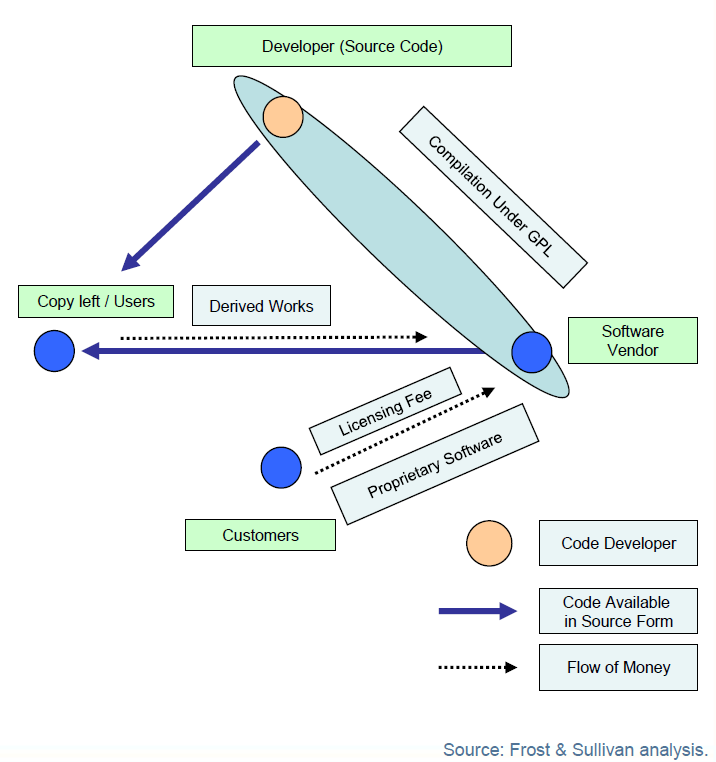
\includegraphics[width=.94\textwidth]{Impact-img1.png}}
%  \caption{The GPL Model}\label{fig:gpl-model}
% \end{figure}

% \begin{figure}[ht]\centering
%  \fbox{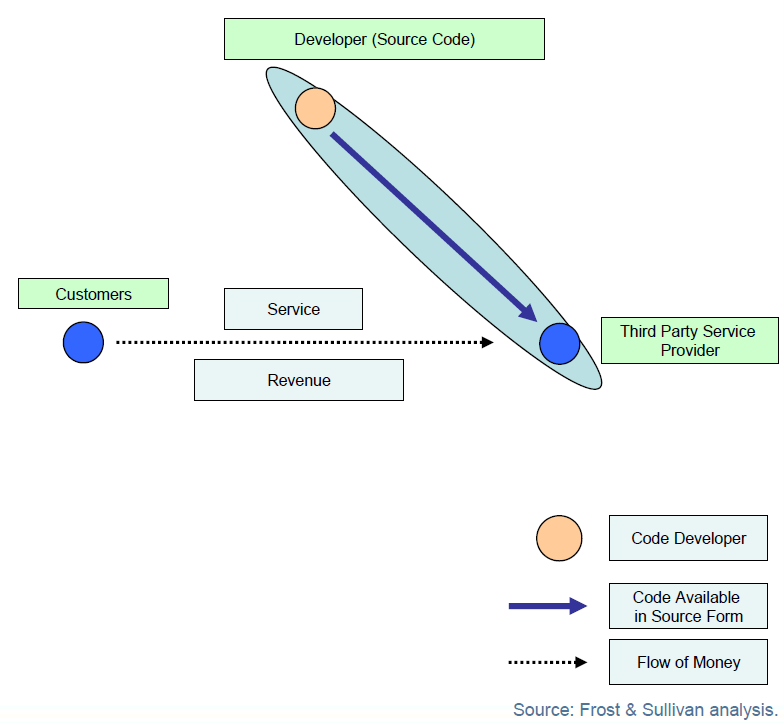
\includegraphics[width=.94\textwidth]{Impact-img2.png}}
%  \caption{The Third-Party Services Model}\label{fig:tps-model}
% \end{figure}

% \begin{compactenum}
% \item The \textbf{GPL model} (see Figure~\ref{fig:gpl-model}): With this model, the vendor
%   is required to make the new code available in source form but it can choose to keep the
%   new code as proprietary and charge for that proprietary software.  The vendor can
%   provide the code commercially as part of a larger platform (hardware/software product)
%   for which the companies receives revenue (license fee for the code + fees for technical
%   support, updates and upgrades).
% \item The \textbf{Third Party Service Model} (see Figure~\ref{fig:tps-model}) Many users
%   may be willing to employ a third party service for distribution, modifications
%   (debugging) and other support.
% \end{compactenum}

\eucommentary{
Where relevant, include information on how the participants will manage
the research data generated and/or collected during the project, in
particular addressing the following issues: What types of data will the
project generate/-collect? What standards will be used? How will this
data be exploited and/or shared/made accessible for verification and
re-use (If data cannot be made available, explain why)? How will this
data be curated and preserved?}

\TOWRITE{E.S. – Nicolas}{, ici je ne peux pas  écrire à ta place. Il faut juste que
tu répondes précisément aux questions posées ci-dessus.}

%Open source software.
%
%
%All software used and/or generated by the project will be Open Source.
%This is a deliberate choice of the project consortium, as commercial
%licenses (and patents) on this type of software only creates barriers
%in our scientific domain.
%
%Benefits of Open Source:
%
%Acquisition and Costs: lower costs, easy access to the infrastructure,
%lower risks of proprietary lock-in
%
%Flexibility: picking up from Open Source projects, reduces dependence on
%supplier, ability to view and modify the source code. Allows peer
%reviewed modifications, community discussions. Open Source provides the
%customer/end user the opportunity to innovate
%
%Support: from developer community.
%
%Besides being cost effective, Open Source software fosters
%reuse, reliability, flexibility, and interoperability.
%
%A consortium agreement will be established to manage ownership and
%access to key knowledge, including software generated by the project.

{\bf Open access policy and data protection.} OpenDreamKit will participate in the Open Research Data Pilot and is fully committed to ensure the open access of relevant project results and data. The consortium will comply with the Guidelines on Open Access to Scientific Publications and Research Data in Horizon 2020. 

The ambitious and interdisciplinary objectives of the project will result in the production of vast amount of research data (we refer to Figure \ref{fig:thebigpicture} and the corresponding subsection for more details). The primary results of the project are expected to take the form of an open-source software, which will be available through the project website and publicly available repositories. Moreover, as the project strives towards efficient integration and representation of various research data and reproducibility of the research results, which represents naturally a challenge, the project will generate a detailed description of the data sources with specifics pertaining to data management (metadata standards, policies for access and sharing and for reuse and distribution, plans for archival and preservation, with accompanying deadlines). This information will be presented in the Data Management Plan, to be delivered within the first six months after the project start and subsequently updated throughout. 

All scientific publications produced in the framework of the project will be either published in open access journals or self-archived using research data repositories. In addition, we will make all experimental data needed to reproduce/validate the results from scientific publications available through research data repositories (e.g. ZENODO, OpenAIRE). 

{\bf Intellectual Property Rights Management.} IPR management will be described in detail in the Consortium Agreement (CA), which will describe all issues regarding the IPR, confidentiality, know-how, rights on exploitation, the rights and obligations of the each partner. The CA will be prepared by the Coordinator, and then signed by all partners before the start of the project. 

Access rights to foreground and background needed for the execution of the project shall be deemed granted, on a royalty-free basis, as of the date of the grant agreement entering into force. Methodology, documents, know-how, software, and tools will be available to all in order to achieve the project objectives during the project lifetime. 

Most of the project results will have joint ownership due to a highly collaborative nature of the project. The CA will specify the terms of the resulting joint ownership, i.e., assignment of shares between joint owners, conditions of use, exploitation and management of jointly used IP. 

The CA will also outline rules for publication procedures to ensure that IP can be protected while minimising publication delay.

The costs related to IPR (including those related to protecting results) and dissemination (i.e., 'gold' open access publications) are included in the project budget of each participating organisation. 

\subsubsection{Communication Activities}
\label{subsubsect:communication}

\eucommentary{Describe the proposed communication measures for promoting the
project and its findings during the period of the grant. Where appropriate
these measures should include social media and public events with user
participation. Measures should be proportionate to the scale of the project,
with clear objectives. They should be tailored to the needs of various audiences,
including groups beyond the project's own community. Where relevant, include
measures for public/societal engagement on issues related to the project.}

Our intention is to increase the attractiveness of mathematics among young generation and females in particular as well as to improve the impact and maximise the visibility of the project activities on the entire VRE ecosystem. The following strategic access points will be used to maximise visibility:

\begin{compactenum}
\item An online presence that explains the OpenDreamKit concept and its applicability in layman's terms and offers significant information (website, social networks, Youtube, press releases).
\item Collaboration with other relevant European and national projects (existing and new ones). We refer to Section \ref{linked-projects} for more details on the linked research and innovation activities.  Presentation of the project results on the annual event 'Worldwide meetings of the free software.' 
\item Collaboration with European and national mathematical societies, e.g., European Mathematical Society, European Women in Mathematics.
\item Presentations/demonstrations at partner institution-specific, locally organised 'science holiday' and 'days of science'.
\item Popularisation papers and communication events addressed to people interested by ICT. 
\item Involvement in workshops / conferences on e-infrastructures and broad mathematical topics, e.g., Swiss Numerical Analysis Day.
\end{compactenum}
%%% Local Variables:
%%% mode: latex
%%% TeX-master: "proposal"
%%% End:

%  LocalWords:  eucommentary programme subsubsection tablehead supertabular hline sur est
%  LocalWords:  e-infrastracture sémantique données amont j'ai mal si répond vraiment ce
%  LocalWords:  critère Systeme flushleft arraybslash Ergonomie il faut réflechir façon
%  LocalWords:  rendre l'outil attractif jeune génération génération des chercheurs va je
%  LocalWords:  définir donc terme Réfléchis possibilité tablettes mais aussi l'enseigner
%  LocalWords:  intéressante textgreater partie suivante demande elle ne serait mieux que
%  LocalWords:  unauthorised Maximise subsubsect organisational Pycon IPython Economie tu
%  LocalWords:  Standartisation Logiciel Libre includegraphics Impact-img1.png peux emph
%  LocalWords:  Impact-img2.png écrire répondes précisément posées ci-dessus TOWRITE fbox
%  LocalWords:  Simula Valeriya textwidth textwidth textbf compactenum longtable Jupyter
%  LocalWords:  organisation organise neighbouring Standartization programmes gpl-model
%  LocalWords:  tps-model thebigpicture Popularisation virtualised organisations Logilab
%  LocalWords:  organisations summarise organising capitalise realising minimising
%  LocalWords:  organised
